\section*{Übung 6}
\subsection*{Aufgabe 1}
\subsubsection*{Lösungsidee}
Es werden alle Fälle in denen Valid False zurückgeben muss, beachtet.
\newline

\lstinputlisting[language=Pascal] {../Ossi.pas}
\begin{figure}[H]
	\centering
	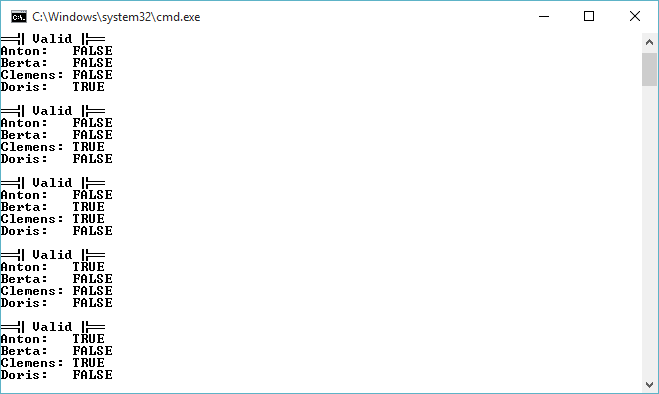
\includegraphics[scale=0.9]{./pictures/Ossi.png}
	\caption{Alle möglichen Kombinationen}
	\label{fig: Ossi Combinations}
\end{figure}

\section*{Testfall}
Zeigt alle möglichen Kombinationen.

\newpage

\subsection*{Aufgabe 2}
\subsubsection*{Lösungsidee}
Die Funktion wird so umgeschrieben das kein Boolean als Rückgabewert verwendet wird. Stattdessen wird -1 und 1 verwendet. 1 wird semantisch als True angesehen und -1 wird semantisch als False angesehen.
\newline

\lstinputlisting[language=Pascal] {../search.pas}
\begin{figure}[H]
	\centering
	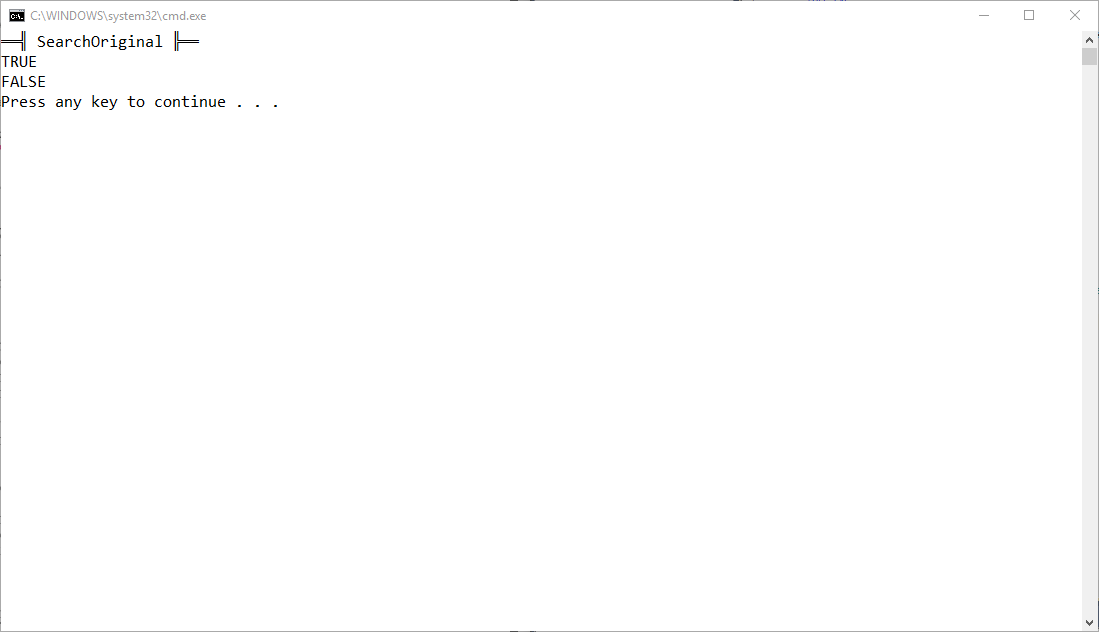
\includegraphics[scale=0.55]{./pictures/Original withoutdirective.png}
	\caption{Testfälle Original ohne Directive}
	\label{fig: Original withoutdirective}
\end{figure}

\begin{figure}[H]
	\centering
	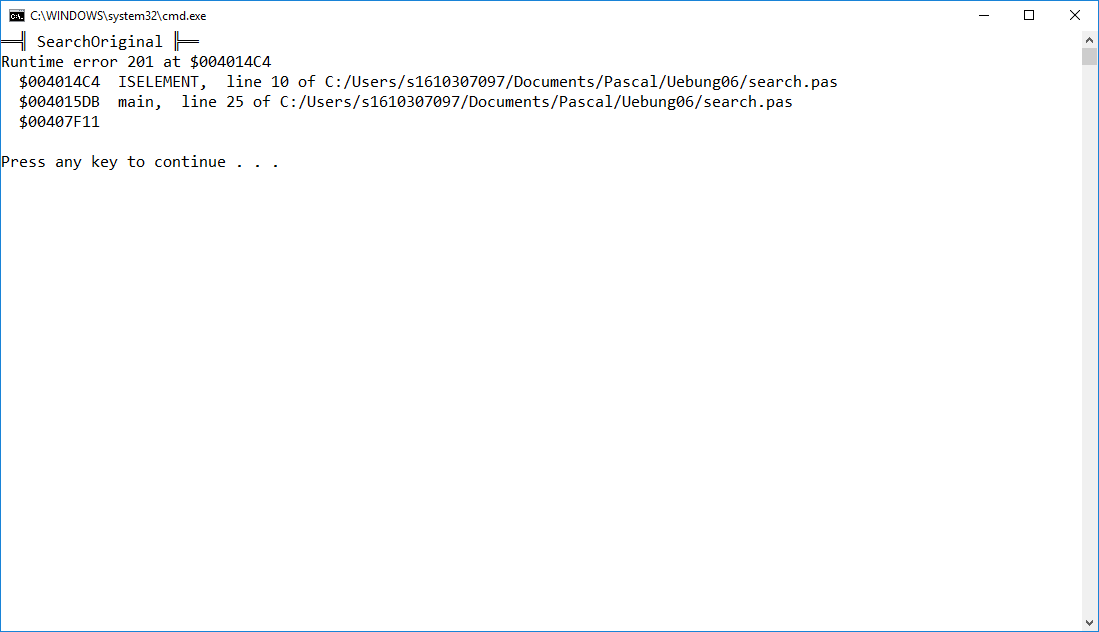
\includegraphics[scale=0.55]{./pictures/Original withdirective.png}
	\caption{Testfälle Original mit Directive}
	\label{fig: Original withdirective}
\end{figure}
\newpage

\lstinputlisting[language=Pascal] {../searchwithoutbool.pas}
\begin{figure}[H]
	\centering
	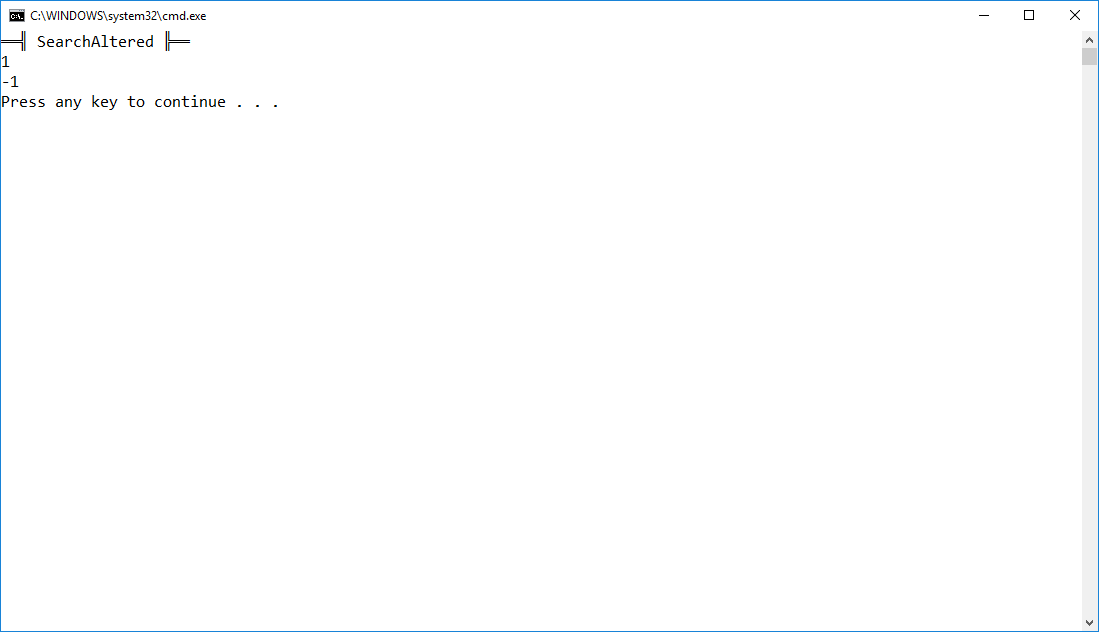
\includegraphics[scale=0.55]{./pictures/Altered with directive.png}
	\caption{Testfälle Suchen mit Directive}
	\label{fig: Search without Bool}
\end{figure}

\section*{Testfälle}
Es werden zwei Zahlen gesucht, eine ist vorhanden die andere nicht (1 wenn gefunden, -1 wenn nicht).

\newpage

\subsection*{Aufgabe 3}
\subsubsection*{Lösungsidee}
Es soll mit Rational Zahlen gerechnet werden. Dazu werden 4 verschieden Procedures verwendet die Multiplizieren, Dividieren, Addieren und Subtrahieren. Nach jeder Operation wird der ggT (größter gemeinsamer Teiler) gesucht und der Bruch vereinfacht. Zusätzlich wird das Rationale Ergebnis ausgegeben.
\newline

\lstinputlisting[language=Pascal] {../rationalcalc.pas}
\begin{figure}[H]
	\centering
	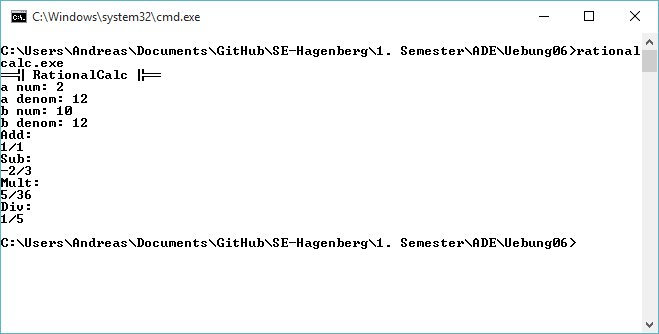
\includegraphics[scale=0.9]{./pictures/rationalcalc1.png}
	\caption{Testfall rationalcalc}
	\label{fig: rationalcalc1}
\end{figure}

\begin{figure}[H]
	\centering
	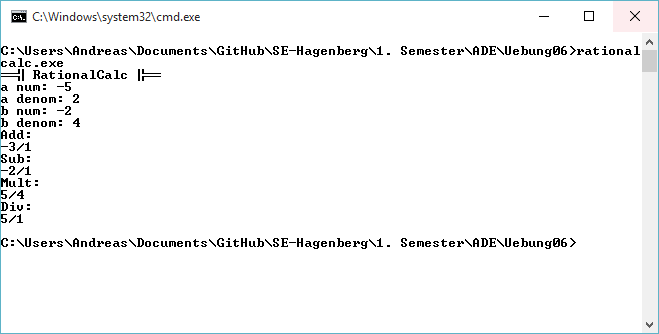
\includegraphics[scale=0.9]{./pictures/rationalcalc3.png}
	\caption{Testfall rationalcalc}
	\label{fig: rationalcalc3}
\end{figure}

\begin{figure}[H]
	\centering
	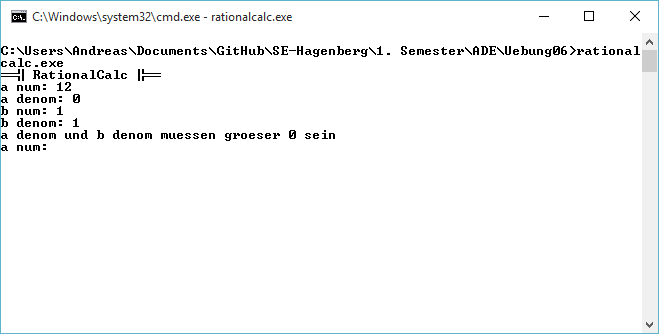
\includegraphics[scale=0.9]{./pictures/rationalcalc2.png}
	\caption{Testfall rationalcalc}
	\label{fig: rationalcalc2}
\end{figure}

\section*{Testfälle}
Die Testfälle zeigen das Rechnen mit zwei verschiedenen Brüchen. Der letzte Testfall zeigt das solange eingelesen wird bis gültige Werte eingegeben wurden.
\newpage